\section{Problem 1 - Data transfer}
\textit{Imaging a new 'huge' memory tag 64kb (or 1Mb?) is used to store personal ID/images (like for passport etc). Is it realistic in a pedestrian set up to perform an 'on the fly' ID retrieval in a automated fashion. I.e. how long time does retrieval take (what interrogator-transponder communication is needed, what duplex form do you consider).. vs typical displacement of a pedestrian in same period of time. Start using Gen1 tag characteristics.. then if need for changes, what sort of tag characteristics would you like? .. where would you look for them/find them?}\\

We assume that the time we have to read a RFID tag from a pedestrian is about 1 second. This gives that if we have a data tag of 64kb in 1 second then we'll need 64kbps data rate to accomplish this. 

\begin{figure}
\centering
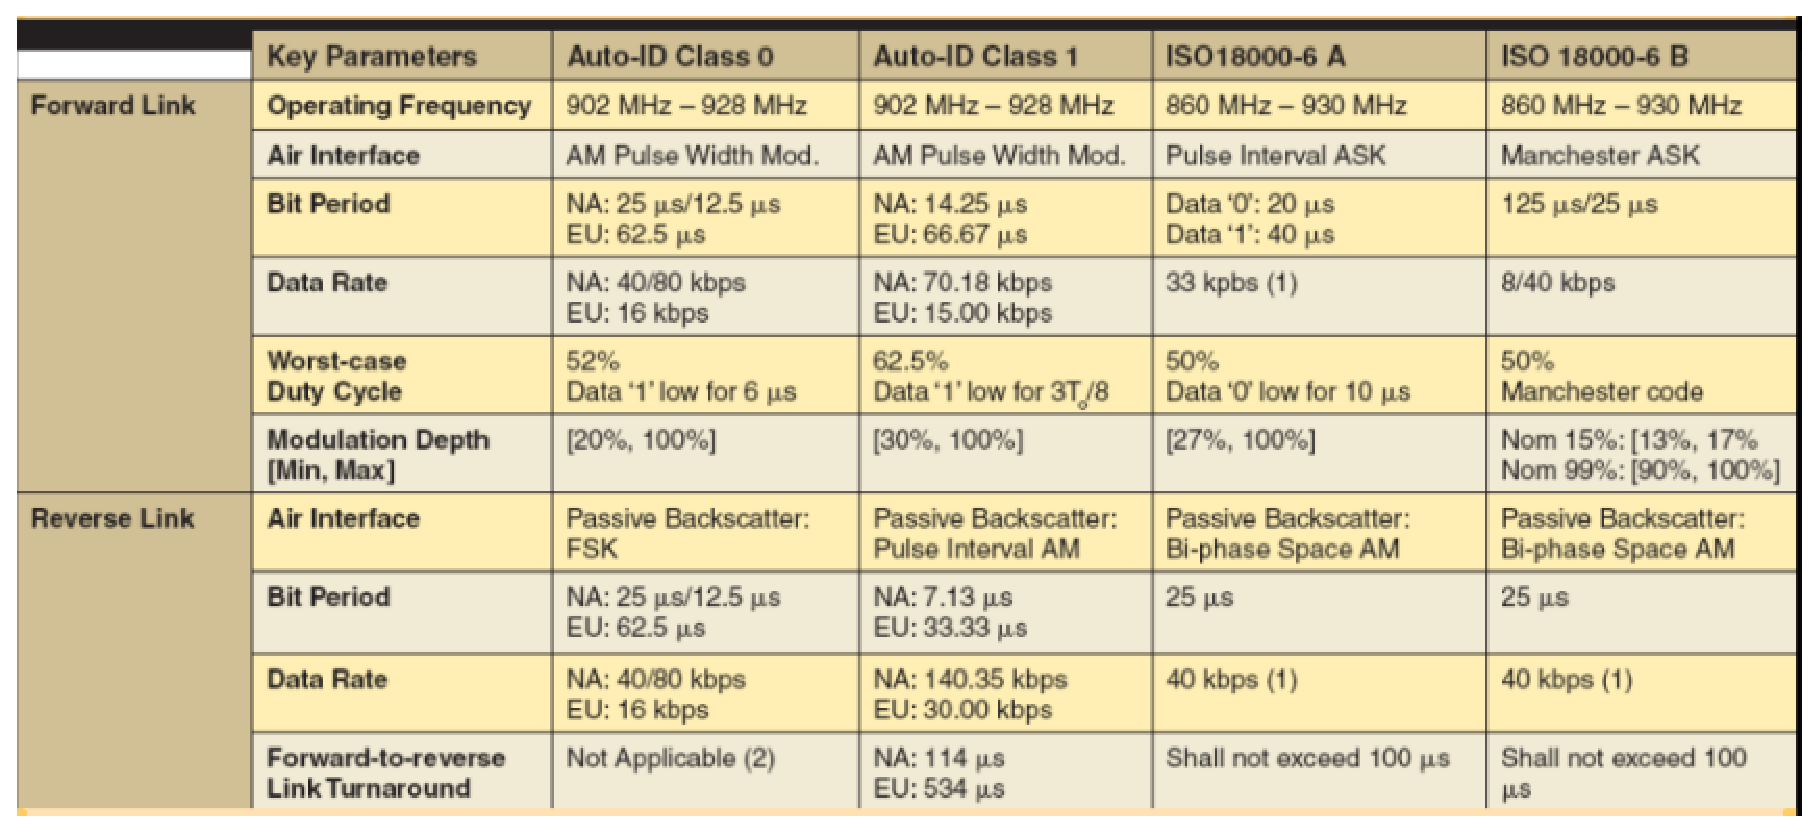
\includegraphics[width=9cm]{mm13-ex1.eps}
\caption{Parameters for different standards}\label{fig:data_rates}
\end{figure}

From \figref{fig:data_rates} it can be seen that none of the ISO 18000-6 standards can afford a data rate that high. In fact the only standard that can transfer data at that speed in the reverse link is the Auto-ID Class1 but just in the North American protocol, being imposible to guarantee the transfer in Europe with any option.\\

If we would have considered that the time to realize the transfer is at least 2 seconds the data rate would be lower than 32kbps what would open the options to the ISO standards in Europe and the rest in North America.\\

For the first generation of RFID there where no authentication for who have access to the data. This is not good for personal information. Therefore a 2nd generation RFID class 2 can be used which have a authentication control system build in. 